\section{函数的基本特征}

函数的基本特征包括: 定义域和值域、解析式与图像、奇偶性、单调性、零点以及渐近线等,这些基本特征可以帮助我们更好地理解和分析函数的性质和行为.

\subsection{函数的主要性质}

\subsubsection{定义域}

\begin{definition}[函数的概念]
    设有两个变量 $x$ 与 $y$,如果变量 $x$ 在其变化范围 $D$ 内任取一个确定的数值时,变量 $y$ 按照一定的规则 $f$,总有唯一确定的数值和它对应,则称变量 $y$ 是变量 $x$ 的\textit{函数},记作 $y=f(x)$,
    $x$ 称为\textit{自变量},$y$ 称为\textit{因变量},$D$ 称为\textit{函数的定义域},$f$ 表示由 $x$ 确定 $y$ 的对应规则.
\end{definition}

\begin{example}
    求函数 $y=\dfrac{1}{\sqrt{25-x^2}}+\arctan\dfrac{x-1}{5}$ 的定义域.
\end{example}
\begin{solution}
    要使函数有意义,变量 $x$ 必须同时满足 $\begin{cases}
        25-x^2>0\\\qty|\dfrac{x-1}{5}|\leqslant 1
    \end{cases}\Rightarrow -4\leqslant x<5$,因此定义域为 $[-4,5).$
\end{solution}

\subsubsection{单调性}

\begin{definition}[函数的单调性]
    设函数 $f(x)$ 的定义域为 $D$,区间 $I\subset D$,对于 $\forall x_1,x_2\in I$,当 $x_1<x_2$ 时,恒有 $f(x_1)<f(x_2)$ (或 $f(x_1)>f(x_2)$) 则称函数 $f(x)$ 在区间 $I$ 上\textit{单调递增 (递减)},
    若 $f(x_1)\leqslant f(x_2)$ (或 $f(x_1)\geqslant f(x_2)$),则称函数 $f(x)$ \textit{单调不减 (不增)}.
\end{definition}
\begin{theorem}[函数的单调性判定]
    设函数 $f(x)$ 在 $[a,b]$ 上连续,在 $(a,b)$ 内可导,如果在区间上有 $f'(x)\geqslant 0(\text{或 }f'(x)\leqslant 0)$ (且不在任一子区间取恒等号),则 $f(x)$ 在 $(a,b)$ 内严格单调递增 (或严格单调递减).
    \index{函数的单调性判定}
\end{theorem}

\begin{example}
    由 $f'(x_0)>0$ 能否得到函数 $f(x)$ 在 $x_0$ 的某个邻域内单调递增?
\end{example}
\begin{solution}
    不能,理由如下:
    利用一阶导数判断函数的单调性,需要已知导数在某区间的正负,而不是某一点导数值的正负
\end{solution}

\subsubsection{奇偶性}

\begin{definition}[函数的奇偶性]
    设函数 $f(x)$ 在关于原点对称的区间 $D$ 上有定义,如果对 $D$ 上任意点 $x$,均有 $f(-x)=f(x)$ (或 $f(-x)=-f(x)$),则称函数 $f(x)$ 为\textit{偶函数 (或奇函数)}.
    奇函数的图像关于原点对称,偶函数的图像关于 $y$ 轴对称.
\end{definition}

\begin{example}[1987 数二]
    $f(x)=|x\sin x|\e^{\cos x}~~(-\infty<x<+\infty)$ 是
    \begin{tasks}(4)
        \task 有界函数
        \task 单调函数
        \task 周期函数
        \task 偶函数
    \end{tasks}
\end{example}
\begin{solution}
    由于 $|x\sin x|$ 和 $\e^{\cos x}$ 都是偶函数,则其乘积 $f(x)=|x\sin x|\e^{\cos x}$ 为偶函数,选 D.
\end{solution}

\subsubsection{周期性}

\begin{theorem}[函数的周期性定理]
    若函数 $f(x)$ 以 $T$ 为周期,则 $$f(x)=f(x+T)=f(x+2T)=\cdots=f(x+nT).$$
    \index{函数的周期性定理}
\end{theorem}

\begin{example}[2014 数一]
    设 $f(x)$ 是周期为 4 的可导奇函数,且 $f'(x)=2(x-1)~ (0\leqslant x\leqslant 2)$,求 $f(7)$.
\end{example}
\begin{solution}
    $f(x)=\displaystyle\int 2(x-1)\dd x=x^2-2x+C$,因为 $f(x)$ 是奇函数,所以 $f(0)=0$,可知 $C=0$,于是 $f(x)=x^2-2x$,
    又 $f(x)$ 的周期为 4,于是 $f(7)=f(-1+8)=f(-1)=-f(1)=1$.
\end{solution}

\subsubsection{有界性}

\begin{theorem}[函数的有界性定理]
    若函数 $f(x)$ 在闭区间 $[a,b]$ 上连续,则 $f(x)$ 在 $[a,b]$ 上有界;
    若函数 $f(x)$ 在开区间 $(a,b)$ 内连续,且 $\displaystyle\lim_{x\to a^+}f(x)$ 与 $\displaystyle\lim_{x\to b^-}f(x)$ 存在,则函数 $f(x)$ 在 $(a,b)$ 内有界.
    \index{函数的有界性定理}
\end{theorem}

\begin{example}[2004 数三]
    函数 $f(x)=\dfrac{|x|\sin(x-2)}{x(x-1)(x-2)^2}$ 在下列哪个区间内有界
    \begin{tasks}(4)
        \task $(-1,0)$
        \task $(0,1)$
        \task $(1,2)$
        \task $(2,3)$
    \end{tasks}
\end{example}
\begin{solution}
    当 $x\neq0,1,2$ 时,$f(x)$ 连续,而
    $$\lim_{x\to-1^+}f(x)=-\dfrac{\sin 3}{18},~\lim_{x\to0^-}f(x)=-\dfrac{\sin 2}{4},~\lim_{x\to0^+}f(x)=\dfrac{\sin 2}{4},~\lim_{x\to1}f(x)=\infty,~\lim_{x\to2}f(x)=\infty$$
    所以函数 $f(x)$ 在 $(-1,0)$ 上有界.
\end{solution}

\subsection{复合函数}

\begin{definition}[复合函数]
    如果我们有两个函数 $ f $ 和 $ g $,而两者的定义域分别是 $ D_{f} $ 和 $ D_{g} $,
    值域分别是 $ I_{f} $ 和 $ I_{g} $. 如果 $ I_{f} \cap D_{g} \neq \varnothing $,
    那我们定义\textit{复合函数}为 $$ g \circ f:=\left\{(x, z) \mid\left(\exists y \in I_{f} \cap D_{g}\right)[y=f(x) \wedge z=g(y)]\right\} .$$
\end{definition}

\begin{example}[2001 数二]
    设 $f(x)=\begin{cases}
            1,|x|\leqslant 1 \\0,|x|>1
        \end{cases}$,则 $f\qty{f[f(x)]}$ 等于
    \begin{tasks}(4)
        \task $0$
        \task $1$
        \task $\begin{cases}
                1,|x|\leqslant 1 \\0,|x|>1
            \end{cases}$
        \task $\begin{cases}
                0,|x|\leqslant 1 \\1,|x|>1
            \end{cases}$
    \end{tasks}
\end{example}
\begin{solution}
    因为 $f\in\qty{0,1}$,所以 $f[f(x)]=1$,那么 $f\qty{1}=1$,因此选 B.
\end{solution}

\begin{theorem}\label{theorem:xn011-1}
    $\displaystyle\lim_{n \to \infty } x^n=\begin{cases}
            0,      & |x|<1         \\
            \infty, & |x|>1         \\
            1,      & x=1           \\
            1,      & x=-1,~n=2k    \\
            -1,     & x=-1,~n=2k+1.
        \end{cases}$
\end{theorem}

\begin{example}
    已知 $f(x)=\displaystyle\lim_{n\to\infty}\sqrt{2+(2x)^n+x^{2n}}~(x\geqslant 0),~g(x)=\lim_{n\to\infty}\dfrac{1-x^{2n+1}}{1+x^{2n}}$,求 $f(g(x))$ 的表达式.
\end{example}
\begin{solution}
    \begin{minipage}{0.7\linewidth}
        由推论 \ref{maxai} 知,$f(x)=\displaystyle\lim_{n\to\infty}\sqrt{1^n+1^n+(2x)^n+(x^2)^{n}}=\max\qty{1,2x,x^2}=\begin{cases}
                1,   & 0\leqslant x<\dfrac{1}{2} \\[6pt]
                2x,  & \dfrac{1}{2}\leqslant x<2 \\[6pt]
                x^2, & 2\leqslant x
            \end{cases}$ 又由定理 \ref{theorem:xn011-1} 可得
        $g(x)=\begin{cases}
                1,  & -1\leqslant x<1 \\
                -x, & |x|>1           \\
                0,  & x=1
            \end{cases}$,于是 $g(x)$ 的图像如图 \ref{fig:IIIgIIfI} 所示,那么
        \begin{flalign*}
            I:  & ~x=1\Rightarrow g(1)=0\Rightarrow f(g(0))=1                                        \\
            II: & ~\begin{cases}
                       -2<x<-1 \\
                       1\leqslant x<1
                   \end{cases}\Rightarrow \begin{cases}
                                              g(x)=-x \\
                                              g(x)=1
                                          \end{cases}\Rightarrow \begin{cases}
                                                                     -x>2 \\
                                                                     -x>1 \\
                                                                     -1\leqslant x<1
                                                                 \end{cases}\Rightarrow \begin{cases}
                                                                                            f(g(x))=x^2 \\
                                                                                            f(g(x))=-2x \\
                                                                                            f(g(x))=2
                                                                                        \end{cases}
        \end{flalign*}
    \end{minipage}\hfill
    \begin{minipage}{0.29\linewidth}
        \begin{figure}[H]
            \centering
            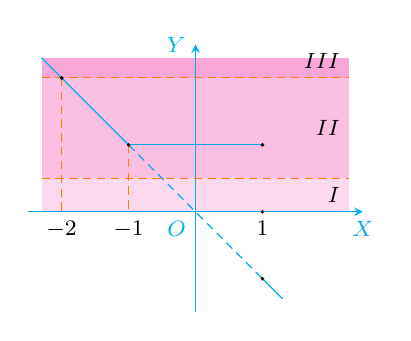
\begin{tikzpicture}[->,samples=100,>=stealth,font=\footnotesize,scale=0.85]
                \fill[magenta!15](-2.3,0)--(2.3,0)--(2.3,0.5)--(-2.3,0.5);
                \fill[magenta!25](-2.3,0.5)--(2.3,0.5)--(2.3,2)--(-2.3,2);
                \fill[magenta!35](-2.3,2)--(2.3,2)--(2.3,2.3)--(-2.3,2.3);
                \draw[->,cyan](-2.5,0)--(0,0)node[below left]{$O$}--(2.5,0)node[below]{$X$};
                \draw[->,cyan](0,-1.5)--(0,2.5)node[left]{$Y$};
                \draw[cyan,-](-2.3,2.3)--(-1,1);
                \draw[cyan,-](1,-1)--(1.3,-1.3);
                \draw[cyan,-](-1,1)--(1,1);
                \draw[densely dashed,orange,-](-2.3,0.5)--(2.3,0.5);
                \draw[densely dashed,orange,-](-2.3,2)--(2.3,2);
                \draw[densely dashed,orange,-](-2,2)--(-2,0);
                \draw[densely dashed,orange,-](-1,1)--(-1,0);
                \draw[densely dashed,cyan,-](-1,1)--(1,-1);
                \node[below] at (-2,0){$-2$};
                \node[below] at (-1,0){$-1$};
                \node[below] at (1,0){$1$};
                \draw[-,fill=black] (-2,2) circle (0.5pt);
                \draw[-,fill=black] (-2,2) circle (0.5pt);
                \draw[-,fill=black] (-1,1) circle (0.5pt);
                \draw[-,fill=black] (1,0) circle (0.5pt);
                \draw[-,fill=white] (1,1) circle (0.5pt);
                \draw[-,fill=white] (1,-1) circle (0.5pt);
                \node[left] at (2.3,0.25){$I$};
                \node[left] at (2.3,1.25){$II$};
                \node[left] at (2.3,2.25){$III$};
            \end{tikzpicture}
            \caption{}
            \label{fig:IIIgIIfI}
        \end{figure}
    \end{minipage}
    $$III:~x\leqslant -2\Rightarrow g(x)=-x\Rightarrow f(g(x))=x^2$$
    综上,$f(g(x))=\begin{cases}
            x^2, & x\leqslant -2   \\
            -2x, & -2<x<-1         \\
            2,   & -1\leqslant x<1 \\
            1,   & x=1.
        \end{cases}$
\end{solution}

\subsection{反函数}

\begin{definition}[反函数]
    设 $f$ 为一函数,其定义域为 $D_f$,值域为 $I_f$,如果存在一函数 $g$,其定义域和值域分别为 $I_g,~D_g$,并对每一 $x\in D_f$ 有:
    $g(f(x))=x$,则称 $g$ 为 $f$ 的\textit{反函数},记为 $f^{-1}.$
    \label{definitionOfInverseFunction}
\end{definition}

\begin{example}
    已知 $g$ 是 $f$ 的反函数,则 $f(2x)$ 的反函数为
    \begin{tasks}(4)
        \task $y=\dfrac{1}{2}g(x)$
        \task $y=2g(x)$
        \task $y=\dfrac{1}{2}g(2x)$
        \task $y=2g(2x)$
    \end{tasks}
\end{example}
\begin{solution}
    令 $y=f(2x)$,反解出 $x:x=\dfrac{1}{2}g(y)$,交换 $x$ 与 $y$ 的位置,于是 $y=\dfrac{1}{2}g(x)$,选 A.
\end{solution}

\begin{example}
    求 $y=\sqrt[3]{x+\sqrt{1+x^{2}}}+\sqrt[3]{x-\sqrt{1+x^{2}}}$ 的反函数表达式.
\end{example}
\begin{solution}
    令 $y_1=\sqrt[3]{x+\sqrt{1+x^{2}}},~y_2=\sqrt[3]{x-\sqrt{1+x^{2}}}$,那么 $y=y_1+y_2$,又因为
    $$y_1^3+y_2^3=(y_1+y_2)\qty(y_1^2-y_1y_2+y_2^2)=(y_1+y_2)\qty[(y_1+y_2)^2-3y_1y_2]$$
    其中 $y_1^3+y_2^3=x+\sqrt{1+x^2}+x-\sqrt{1+x^2}=2x,~y_1y_2=\sqrt[3]{x^2-1-x^2}=-1$,因此 $$2x=y\qty(y^2+3)\Rightarrow x=\dfrac{y\qty(y^2+3)}{2}.$$
\end{solution}

\begin{example}
    设 $f(x)=2023x^{2023}+x+1,~f^{-1}(x)$ 是 $f(x)$ 的反函数,计算极限 $$\lim_{x\to+\infty}\dfrac{f^{-1}(2023x)-f^{-1}(x)}{\sqrt[2023]{x}}.$$
\end{example}
\begin{solution}
    设 $g(x)=f^{-1}(x)$,由定义 \ref{definitionOfInverseFunction},得 $f(g(x))=x$,于是 $$x=2023 g^{2023}(x)+g(x)+1$$
    则 $$\lim_{x\to+\infty}\dfrac{f^{-1}(x)}{\sqrt[2023]{x}}=\lim_{x\to+\infty}\dfrac{g(x)}{\sqrt[2023]{2023x^{2023}+g(x)+1}}=\lim_{x\to+\infty}\dfrac{1}{\sqrt[2023]{2023+\dfrac{1}{g^{2022}(x)}+\dfrac{1}{g^{2023}(x)}}}=\dfrac{1}{\sqrt[2023]{2023}}$$
    进而有
    $$\lim_{x\to+\infty}\dfrac{f^{-1}(2023x)}{\sqrt[2023]{x}}=\lim_{x\to+\infty}\dfrac{f^{-1}(2023x)}{\sqrt[2023]{2023x}}\cdot\dfrac{\sqrt[2023]{2023x}}{\sqrt[2023]{x}}=\dfrac{\sqrt[2023]{2023}}{\sqrt[2023]{2023}}=1$$
    故原极限为 $1-\dfrac{1}{\sqrt[2023]{2023}}.$
\end{solution}


\subsection{函数的连续性及间断点的类型}

\subsubsection{连续函数}

\begin{definition}[函数连续]
    若 $\displaystyle\lim_{x\to x_0}f(x)=f(x_0)$,则称函数 $f(x)$ 在点 $x_0$ 处连续,若函数 $f(x)$ 在区间 $ I $ 内每一点都连续,则称函数 $f(x)$ 在区间 $I$ 内\textit{连续}.
\end{definition}

\begin{definition}[单侧连续]
    若 $\displaystyle\lim_{x\to x_0^-}f(x)=f(x_0)$,则称函数 $f(x)$ 在 $x_0$ 处\textit{左连续}; 若 $\displaystyle\lim_{x\to x_0^+}f(x)=f(x_0)$,则称函数 $f(x)$ 在 $x_0$ 处\textit{右连续}.
\end{definition}

\begin{theorem}[函数连续的充要条件]
    $f(x)$ 在点 $x_0$ 处连续等价于 $f(x)$  在点 $x_0$ 处既左连续又右连续.
    \index{函数连续的充要条件}
\end{theorem}

\subsubsection{第一类间断点}

\begin{definition}[可去间断点]
    如果不连续点 $ x_{0} $ 两侧函数的极限存在且相等,无论在 $ x_{0} $ 处是否定义
    (若有定义,则函数值不是在这一点的左右极限),
    这类间断点叫\textit{可去间断点} (或可移间断点),这类函数通过补充定义
    $$f\left(x_{0}\right)=\lim _{x \rightarrow x_{0}^{+}} f(x)=\lim _{x \rightarrow x_{0}^{-}} f(x)$$
    后可变为连续函数.
\end{definition}

\begin{definition}[跳跃间断点]
    如果不连续点 $x_{0}$ 两侧函数的极限存在但不相等,称函数在这些点是\textit{跳跃间断点}.
\end{definition}

\subsubsection{第二类间断点}

所有不是第一类间断点的类型,都是第二类间断点.

\begin{definition}[无穷间断点]
    函数在某点的左右极限至少有一个是无穷,这样的间断点就是\textit{无穷间断点},由此可知函数在这个间断点的某个邻域中无界. 无穷间断点的一个重要特性是它是必不可积的.
\end{definition}
% 可参考例题 \ref{fxdfracx12x1}.

\begin{definition}[振荡间断点]
    对于一个函数,当自变量趋于某一点时,函数值在两个常数间变动无限多次,这时函数在这一点处不存在有限极限也不是无穷.
    这样的间断点是\textit{振荡间断点},由此可知函数在这个间断点的某个邻域中有界. 振荡间断点的一个重要特性是它可能是可积的.
\end{definition}

\begin{example}
    设 $f(x)=\dfrac{\qty(1-2^{\frac{1}{x-1}})\e^{\frac{1}{x}}}{1+2^{\frac{2}{x-1}}}\cdot\arctan\dfrac{[~x+1~]}{x+1}$,则下列关于 $f(x)$ 间断点的描述正确的是
    \begin{tasks}(1)
        \task $f(x)$ 有一个可去间断点,一个跳跃间断点,一个第二类间断点
        \task $f(x)$ 有两个可去间断点,一个第二类间断点
        \task $f(x)$ 有两个跳跃间断点,一个第二类间断点
        \task $f(x)$ 有一个跳跃间断点,两个第二类间断点
    \end{tasks}
\end{example}
\begin{solution}
    因为 $x\neq-1,0,1$,下求各不连续点的左右极限值,
    $$f(-1^-)=\lim_{x\to-1^-}f(x)=\lim_{\substack{x\to-1-\delta\\\delta>0}}f(x)=\dfrac{\qty(1-2^{-\frac{1}{2}})\e^{-1}}{1+2^{-1}}\cdot\dfrac{\pi}{2},~f(-1^+)=\lim_{x\to-1^+}=\lim_{\substack{x\to-1+\delta\\\delta>0}}f(x)=0$$
    则 $x=-1$ 为 $f$ 的跳跃间断点;
    $$f(0^-)=\lim_{x\to0^-}f(x)=\lim_{\substack{x\to0-\delta\\\delta>0}}f(x)=0,~f(0^+)=\lim_{x\to0^+}f(x)=\lim_{\substack{x\to0+\delta\\\delta>0}}f(x)=+\infty$$
    则 $x=0$ 为 $f$ 的第二类间断点;
    $$f(1^-)=\lim_{x\to1^-}f(x)=\lim_{\substack{x\to1-\delta\\\delta>0}}f(x)=\e\cdot\arctan\dfrac{1}{2},~f(1^+)=\lim_{x\to1^+}f(x)=\lim_{\substack{x\to1+\delta\\\delta>0}}f(x)=0$$
    则 $x=1$ 为 $f$ 的跳跃间断点,故选 C.
\end{solution}

\subsection{渐近线方程}

\begin{definition}[铅直渐近线]
    若 $\displaystyle\lim_{x\to\varepsilon^-}f(x)$ 与 $\displaystyle \lim_{x\to\varepsilon^+}f(x)$ 至少有一个为无穷大,则称 $x=\varepsilon$ 为曲线 $y=f(x)$ 的\textit{铅直渐近线}.
\end{definition}
\begin{definition}[水平渐近线]
    若 $\displaystyle\lim_{x\to-\infty}f(x)=b$ 或 $\displaystyle\lim_{x\to+\infty}f(x)=b$,其中 $b$ 为常数,则称 $y=b$ 为曲线 $y=f(x)$ 的\textit{水平渐近线}.
\end{definition}
\begin{definition}[斜渐近线]
    若 $\displaystyle\lim_{x\to-\infty}\dfrac{f(x)}{x}=k$ 存在且不为零,同时 $\displaystyle\lim_{x\to-\infty}[f(x)-kx]=b$ 也存在 (或 $\displaystyle\lim_{x\to+\infty}\dfrac{f(x)}{x}=k$ 存在且不为零,同时 $\displaystyle\lim_{x\to+\infty}[f(x)-kx]=b$ 存在),
    则称 $y=kx+b$ 为曲线 $y=f(x)$ \textit{斜渐近线}.
\end{definition}

\begin{example}
    求下列曲线的全部渐近线.
    \setcounter{magicrownumbers}{0}
    \begin{table}[H]
        \centering
        \begin{tabular}{l | l}
            (\rownumber{}) $y=\sqrt{4x^2+x}\ln\qty(2+\dfrac{1}{x}).$ & (\rownumber{}) $y=\mathrm{e}^{x^{-2}}\arctan\dfrac{x^2+x+1}{(x-1)(x+2)}.$                  \\
            (\rownumber{}) $y=\dfrac{x^3}{(x-1)^2}\cos(2\arctan x).$ & (\rownumber{}) $\displaystyle y=(2x+1)\arctan x+\dfrac{\arctan\dfrac{1}{x^2-1}}{x^2+x-2}.$ \\
            (\rownumber{}) $y^3=x\qty(x^2-2y).$                      & (\rownumber{}) $x^3-y^3=6xy.$
        \end{tabular}
    \end{table}
\end{example}
\begin{solution}
    \begin{enumerate}[label=(\arabic{*})]
        \item 由 $\displaystyle\lim_{x\to\qty(-\frac{1}{2})^+}y=-\infty$,且 $\displaystyle\lim_{x\to0^-}y=0$,所以曲线存在一条铅直渐近线 $x=-\dfrac{1}{2}$,又
              \begin{flalign*}
                  k & =\lim_{x\to+\infty}\dfrac{y}{x}=\lim_{x\to+\infty}\dfrac{\sqrt{4x^2+x}}{x}\ln\qty(2+\dfrac{1}{x})=\lim_{x\to+\infty}\dfrac{|x|}{x}\sqrt{4+\dfrac{1}{x}}\ln\qty(2+\dfrac{1}{x})=2\ln 2 \\
                  b & =\lim_{x\to+\infty}(y-kx)=\lim_{x\to+\infty}\qty[\sqrt{4x^2+x}\ln\qty(2+\dfrac{1}{x})-2\ln 2x]                                                                                        \\
                    & =\lim_{x\to+\infty}\qty[\sqrt{4x^2+x}\ln 2-2\ln 2\cdot x+\sqrt{4x^2+x}\ln\qty(2+\dfrac{1}{x})-\sqrt{4x^2+x}\ln 2]                                                                     \\
                    & =\lim_{x\to+\infty}\qty[\dfrac{x}{\sqrt{4x^2+x}+2x}\cdot\ln 2 +|x|\sqrt{4+\dfrac{1}{x}}\ln\qty(1+\dfrac{1}{2x})]=\dfrac{1}{4}\ln 2+1
              \end{flalign*}
              故存在一条斜渐近线方程 $y=2\ln 2x+\dfrac{1}{4}\ln 2+1$,同理当 $x\to-\infty$ 时,也存在一条斜渐近线方程 $$y=-2\ln 2x-\dfrac{1}{4}\ln 2-1.$$
        \item 由 $\displaystyle \lim_{x\to-2^-}y=\dfrac{\pi}{2\mathrm{e}^4},~\lim_{x\to-2^+}y=-\dfrac{\pi}{2\mathrm{e}^4},~\lim_{x\to1^-}y=-\dfrac{\pi\mathrm{e}}{2},~\lim_{x\to1^+}y=\dfrac{\pi\mathrm{e}}{2},~\lim_{x\to0^-}y=-\infty$,故 $y$ 的铅直渐近线为 $x=0$,因为
              $$\lim_{x\to-\infty}y=\lim_{x\to+\infty}y=\lim_{x\to\infty}y=\lim_{x\to\infty}\mathrm{e}^{x^{-2}}\arctan\dfrac{1+\dfrac{1}{x}+\dfrac{1}{x^2}}{1+\dfrac{1}{x}-\dfrac{2}{x^2}}=\dfrac{\pi}{4}$$
              故 $y$ 的水平渐近线为 $y=\dfrac{\pi}{4}$,又因为
              $$k=\lim_{x\to+\infty}\dfrac{y }{x}=\lim_{x\to+\infty}\dfrac{\mathrm{e}^{-x^2}}{x}\arctan\dfrac{x^2+x+1}{(x-1)(x+2)}=0$$
              故曲线共存在两条渐近线,分别为 $x=0$ 与 $y=\dfrac{\pi}{4}$.
        \item 显然 $x=1$ 为该曲线的铅直渐近线,下求斜渐近线,
              \begin{flalign*}
                  k & =\lim_{x\to\pm\infty}\dfrac{y}{x}=\lim_{x\to\pm\infty}\dfrac{x^2}{(x-1)^2}\cos(2\arctan x)=1\cdot -1=-1                                               \\
                  b & =\lim_{x\to\pm\infty}(y-kx)=\lim_{x\to\pm\infty}\dfrac{x^3\cos(2\arctan x)+x(x-1)^2}{(x-1)^2}=\lim_{x\to\pm\infty}\dfrac{-x^3+x^3-2x^2+x}{(x-1)^2}=-2
              \end{flalign*}
              所以斜渐近线方程为 $y=-x-2.$
        \item 因为 $\displaystyle\lim_{x\to\infty}f(x)=\infty$,所以曲线 $y=f(x)$ 没有水平渐近线; 由 $\displaystyle\lim_{x\to-2}f(x)=\infty$,得 $x=-2$ 为曲线 $y=f(x)$ 的铅直渐近线;
              由 $$f(-1^-)=\lim_{x\to-1^-}f(x)=\dfrac{\pi}{4}-\dfrac{\pi}{4}=0,~f(-1^+)=\lim_{x\to-1^+}f(x)=\dfrac{\pi}{4}+\dfrac{\pi}{4}=\dfrac{\pi}{2}$$
              得 $x=-1$ 不是该曲线的铅直渐近线;
              又由 $$\lim_{x\to1}f(x)=\dfrac{3\pi}{4}+\lim_{x\to1}\dfrac{\arctan\dfrac{1}{x^2-1}}{x^2+x-2}=\infty$$
              得 $x=1$ 是该曲线的铅直渐近线; 下求斜渐近线,
              $$k_1=\lim_{x\to-\infty}\dfrac{f(x)}{x}=\lim_{x\to-\infty}\qty(2+\dfrac{1}{x})\arctan x+\dfrac{\arctan\dfrac{1}{x^2-1}}{x^3+x^2-2x}=-\pi$$
              那么
              \begin{flalign*}
                  b_1 & =\lim_{x\to-\infty}\qty(f(x)-kx)=\lim_{x\to-\infty}\qty[(2x+1)\arctan x+\dfrac{\arctan\dfrac{1}{x^2-1}}{x^2+x-2}+\pi x]                                      \\
                      & =2\lim_{x\to-\infty}x\qty(\arctan x+\dfrac{\pi}{2})+\lim_{x\to-\infty}\arctan x+\lim_{x\to-\infty}\dfrac{\arctan\dfrac{1}{x^2-1}}{x^2+x-2}=-\dfrac{\pi}{2}-2
              \end{flalign*}
              那么一条斜渐近线为 $y=-\pi x-\dfrac{\pi}{2}-2$,同理可求解另一条斜渐近线为 $y=\pi x+\dfrac{\pi}{2}-2.$
        \item 令 $k=\dfrac{y}{x}$,有 $$k^3\cdot x^3=x\qty(x^2-2kx)\Rightarrow k^3=1-\dfrac{2k}{x}$$
              两边取极限有
              \begin{flalign*}
                  \lim_{x\to\pm\infty}k^3=\lim_{x\to\pm\infty}\qty(1-\dfrac{2k}{x}) \Rightarrow\lim_{x\to\pm\infty}k^3=\lim_{x\to\pm\infty}\qty(1-2k\cdot\dfrac{1}{x})\Rightarrow k=1
              \end{flalign*}
              令 $b=y-kx=y-x$,那么
              $$(x+b)^3=x\qty(x^2-2x+2b)\Rightarrow \dfrac{b^3}{x^2}+3b+\dfrac{3b^2}{x}=-2\dfrac{b}{x}-2$$
              两边取极限有
              $$\lim_{x\to\pm\infty}\qty(\dfrac{b^3}{x^2}+3b+\dfrac{3b^2}{x})=\lim_{x\to\pm\infty}\qty(-2\dfrac{b}{x}-2)$$
              解得 $b=-\dfrac{2}{3}$,于是斜渐近线方程为 $y=x-\dfrac{2}{3}.$
        \item 令 $y=tx$,代入原方程得 $\begin{cases}
                      x=\dfrac{6t}{1-t^3} \\[6pt]
                      y=\dfrac{6t^2}{1-t^3}
                  \end{cases}$ 当 $x\to\infty$ 时,$\dfrac{6t}{1-t^3}\to\infty\Rightarrow t\to 1$,并且此时 $y\to\infty$,因此
              \begin{flalign*}
                  k & =\lim_{x\to\infty}\dfrac{y}{x}=\lim_{t\to 1}\dfrac{6t^2}{1-t^3}\cdot\dfrac{1-t^3}{6t}=\lim_{t\to1}t=1           \\
                  b & =\lim_{x\to\infty}(y-kx)=\lim_{t\to1}\dfrac{6t^2-6t}{1-t^3}=6\lim_{t\to1}\dfrac{t(t-1)}{-(t-1)\qty(t^2+t+1)}=-2
              \end{flalign*}
              因此该曲线的斜渐近线为 $y=x-2.$
              %\textbf{法二: }转化为射影平面上齐次坐标方程 $S(x,y,z)=x^3-y^3-6xyz=0$,曲线上任取一点 $P(x_0,y_0,z_0)$ 处切线的齐次坐标为
              %      $$\grad S(P)=\qty(\pdv{S}{x},\pdv{S}{y},\pdv{S}{z})\biggl |_{P}=\qty(x_0^2-2y_0z_0,-y_0^2-2x_0z_0,-2x_0y_0)$$
              %      在曲线无穷远处 $z_0=0$,代入曲线方程有 $$x_0^3-y_0^3=0\Rightarrow x_0=y_0\neq0$$
              %      所以此处切线方程的齐次坐标为 $\qty(x_0^2,-x_0^2,-2x_0^2)=(1,-1,2)$
              %      因此切线为实射影直线 $x-y+2z=0$,
              %      令 $z=1$ 时转化为欧氏平面方程 $x-y+2=0$ 即为所求的渐近线方程.
    \end{enumerate}
\end{solution}

\begin{theorem}[割线定理]
    \begin{enumerate}[label=(\arabic{*})]
        \item 设 $ p>0 $,$ y=f(x) $ 在 $ [p,+\infty) $ 上有界,若有
              $$\begin{array}{l}
                      \displaystyle\lim _{x \rightarrow+\infty}[f(x+1)-f(x)]=k, \\
                      \displaystyle\lim _{x \rightarrow+\infty}[(x+1) f(x)-x f(x+1)]=b
                  \end{array}$$
              则直线 $ y=k x+b $ 是曲线 $ y=f(x) $ 的渐近线.
        \item 设 $ q<0 $,$ y=f(x) $ 在 $ (-\infty, q] $ 上有界,若有
              $$\begin{array}{l}
                      \displaystyle \lim _{x \rightarrow+\infty}[f(x+1)-f(x)]=k, \\
                      \displaystyle \lim _{x \rightarrow+\infty}[(x+1) f(x)-x f(x+1)]=b,
                  \end{array}$$
              则直线 $ y=k x+b $ 是曲线 $ y=f(x) $ 的渐近线.
    \end{enumerate}
    \index{割线定理}
\end{theorem}

\begin{example}[2023 数一]
    求曲线 $y=x\ln\qty(\mathrm{e}+\dfrac{1}{x-1})$ 的斜渐近线方程.
\end{example}
\begin{solution}
    \textbf{法一: }渐近线的斜率为 $$k=\lim_{x\to\infty}\dfrac{y}{x}=\lim_{x\to\infty}\ln\qty(\mathrm{e}+\dfrac{1}{x-1})=1$$
    渐近线的截距为 $$b=\lim_{x\to\infty}[f(x)-kx]=\lim_{x\to\infty}\qty[x\ln\qty(\mathrm{e}+\dfrac{1}{x-1})-x]=\lim_{x\to\infty}x\ln\qty[1+\dfrac{1}{\mathrm{e}(x-1)}]=\lim_{x\to\infty}\dfrac{x}{\mathrm{e}(x-1)}=\dfrac{1}{\mathrm{e}}$$
    故所求斜渐近线方程为 $y=x+\dfrac{1}{\mathrm{e}}$.\\
    \textbf{法二: }改写函数表达式为 $$y=x\ln\mathrm{e}\qty[1+\dfrac{1}{\mathrm{e}(x-1)}]=x+x\ln\qty[1+\dfrac{1}{\mathrm{e}(x-1)}]=x+\dfrac{x}{\mathrm{e}(x-1)}=x+\dfrac{1}{\mathrm{e}}+o(1)~  (x\to\infty)$$
    所以斜渐近线方程为 $y=x+\dfrac{1}{\mathrm{e}}.$\\
    \textbf{法三: }利用割线定理,
    \begin{flalign*}
        k & =\lim_{x\to\infty}\qty[f(x+1)-f(x)]=\lim_{x\to\infty}\qty[(x+1)\ln\qty(\e+\dfrac{1}{x})-x\ln\qty(\e+\dfrac{1}{x-1})]=1+\lim_{x\to\infty}x\ln\dfrac{\e+x^{-1}}{\e+(x-1)^{-1}}                                                 \\
          & =1+\lim_{x\to\infty}x\cdot\dfrac{\dfrac{1}{x}-\dfrac{1}{x-1}}{\e+\dfrac{1}{x-1}}=1-\lim_{x\to\infty}\dfrac{1}{\e(x-1)+1}=1                                                                                                   \\
        b & =\lim_{x\to\infty}\qty[(x+1)f(x)-xf(x+1)]=\lim_{x\to\infty}\qty[(x+1)x\ln\qty(\e+\dfrac{1}{x-1})-x(x+1)\ln\qty(\e+\dfrac{1}{x})]                                                                                             \\
          & =\lim_{x\to\infty}x(x+1)\ln\dfrac{\e+\dfrac{1}{x}-\dfrac{1}{x}+\dfrac{1}{x-1}}{\e+\dfrac{1}{x}}=\lim_{x\to\infty}x(x+1)\dfrac{\dfrac{1}{x-1}-\dfrac{1}{x}}{\e+\dfrac{1}{x}}=\lim_{x\to\infty}\dfrac{x}{\e x+1}=\dfrac{1}{\e}
    \end{flalign*}
    因此该曲线的斜渐近线为 $y=x+\dfrac{1}{\e}.$
\end{solution}
